\documentclass[article]{BJTU-thesis}
\usepackage{url}
\usepackage{booktabs}
\setcounter{tocdepth}{4}
\setcounter{secnumdepth}{4}
\hypersetup{hidelinks}
\renewcommand\thesection{\arabic {section}}
\renewcommand\thefigure{\arabic {figure}}
\definecolor{mygreen}{rgb}{0.15,0.66,0.7}
\definecolor{myblue}{rgb}{0,0,164}
\definecolor{mygray}{rgb}{0.6,0.65,0.74}
\definecolor{mymauve}{rgb}{0.58,0,0.82}
\lstset{
	numbers=left, 
	breaklines=true,              
	columns=fixed, 
	commentstyle=\color{mygray}\rmfamily\itshape,    
	keywordstyle=\color{myblue},    
	stringstyle=\color{mygreen}\ttfamily,  
	rulesepcolor=\color{red!20!green!20!blue!20} }

%%%%%%%%%%%%%%%填写封面信息%%%%%%%%%%%%%%%%%%%%
\authora{汤新宇  17301137}
\authorb{陈嘉琪  17301060}
\authorc{刘歆怡  17301129}
\authord{唐{\color{white}哈}麒  17301138}
\authorf{张钰铎  17301145}
\comment{同{\color{white}哈}等{\color{white}哈}贡{\color{white}哈}献}
%\studentNumber{16121248}
\advisor{冀振燕}
%\advisorTitle{教授}
%\degreeType{学术型}
%\major{机械制造}
%\researchArea{切削力分析}
\title{OWL 入侵监测系统架构设计}
\bibliographystyle{unsrt} % BibTex
%\englishtitle{The Path Planning of Blade Machining Tool Based on Cutting Force Analysis.}
%%%%%%%%%%%%%%%%%%%%%%%%%%%%%%%%%%%%%%%%%%%%%%
%\setmainfont{Times New Roman}
\bibliographystyle{unsrt} % BibTex
\begin{document}
	\makecover
	
	\tableofcontents
	\newpage

	\newpage
	\setcounter{page}{1}
	\section{系统简介}
	近年来,随着计算机视觉和网络技术的发展,互联网+安防的应用场景逐渐走进了大众的视野。例如基于实时的视频流,利用图像识别功能,自动检测视频中的运动物体,通过包括后端数据处理和前端 web 页面实时显示结果的系统,被广泛应用在小区入侵监测、智能家居的安防和老人智能看护等领域。在此基础上,加入人脸识别系统,结合其他的智能产品,即可实现高度自动化的物联网自动化运行环境。此外,借助云计算技术,将异常图像上传至云服务器,配合手机APP,可实达到全方位、实时监控的目的。
	
	本项目拟借助 Raspberry Pi 和 Pi camera 模拟应用场景中的监控设备,在监控端、服务器和前端网页之间通过 WebSocket 进行数据传输,实现仓库管理场景下的实时监控、入侵监测等功能。系统概貌如\textbf{图\ref{fig:fig1}}所示,开发环境如\textbf{表\ref{tab:tab1}}所示。
	
	\begin{figure}[!htb]
		\centering
		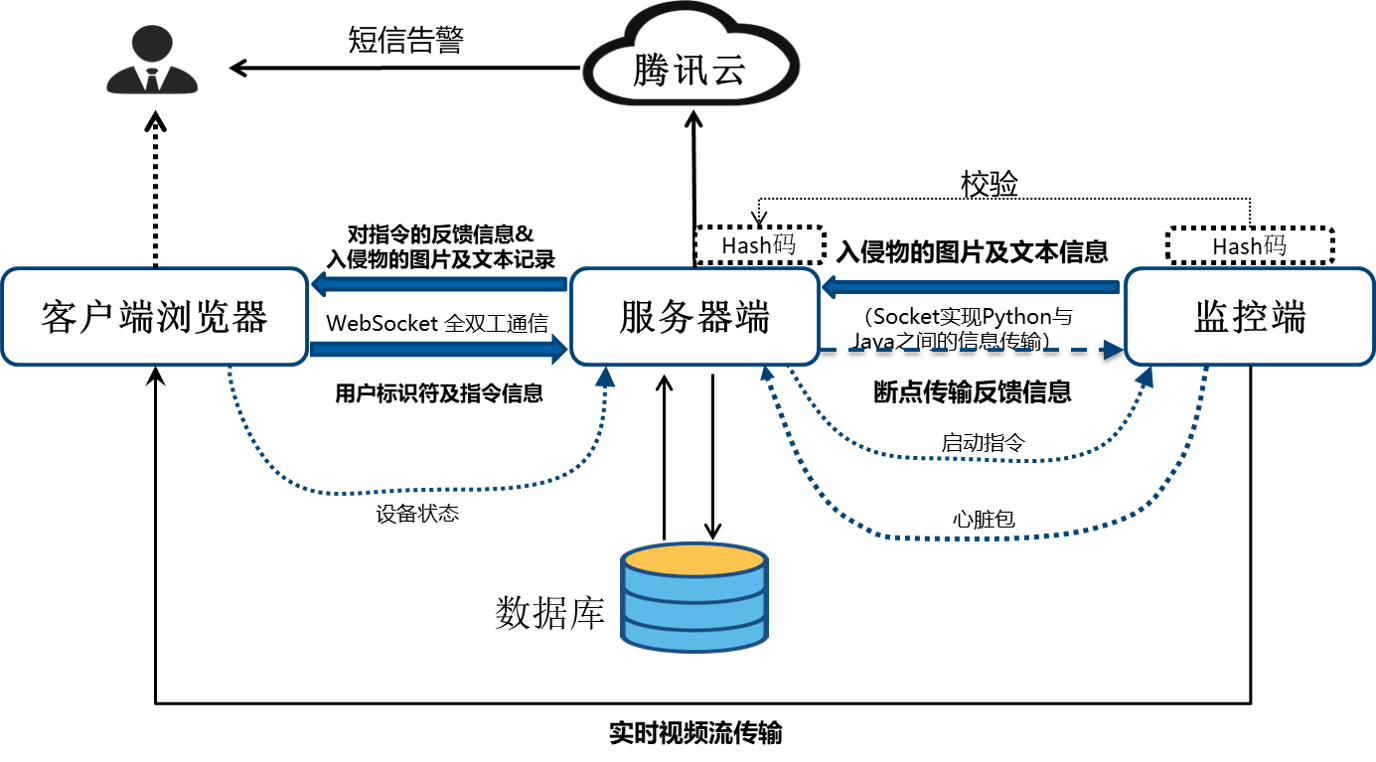
\includegraphics[scale=0.6]{img/1.png}
		\caption{系统概貌图}\label{fig:fig1}
	\end{figure}

	\begin{table}[!htbp]
		\centering
		\caption{开发环境表}
		\label{tab:tab1}
		\begin{tabular}{|c|c|c|}
			\hline
			& 名称 & 版本 \\ \hline
			操作系统 & Windows 10 & Windows SDK 10.0.17763.0 \\ \hline
			数据库 & MySQL & 8.0.16 \\ \hline
			监控端 & Python & 3.5 \\ \hline
			服务器端 & Java & JDK 8 \\ \hline
			客户端 & Vue、Nuxt.js &  \\ \hline
		\end{tabular}
	\end{table}
	
	
\section{功能描述}
\subsection{监控端}
\begin{figure}[!htbp]
	\centering
	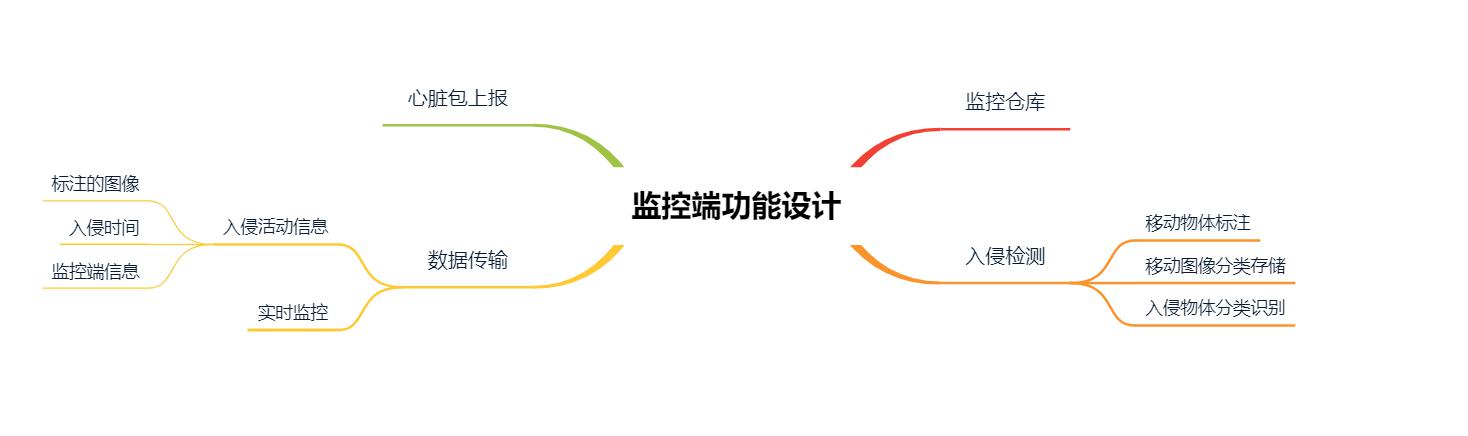
\includegraphics{img/2.jpg}
	\caption{监控端功能示意图}\label{fig:fig2}
\end{figure}

如\textbf{图\ref{fig:fig2}}所示,监控端的主要功能需求为
\begin{enumerate}
	\item 在完成监控端设备的安装和配置后,监控端通过外置镜头对仓库
	进行基本监控功能;
	\item 通过 Background subtraction 方法对视野范围内的画面进行移动物体监测,对移动物体进行标注和分类存储;
	\item 将监测到的入侵活动,以包含设备序列号、时间、入侵物体分类和异常图片及其哈希值等的数据包向服务器传输;
	\item 对实时监控视频流进行编码并传输;
	\item 传输心脏包。
\end{enumerate}

\subsection{服务器}
\begin{figure}[!htbp]
	\centering
	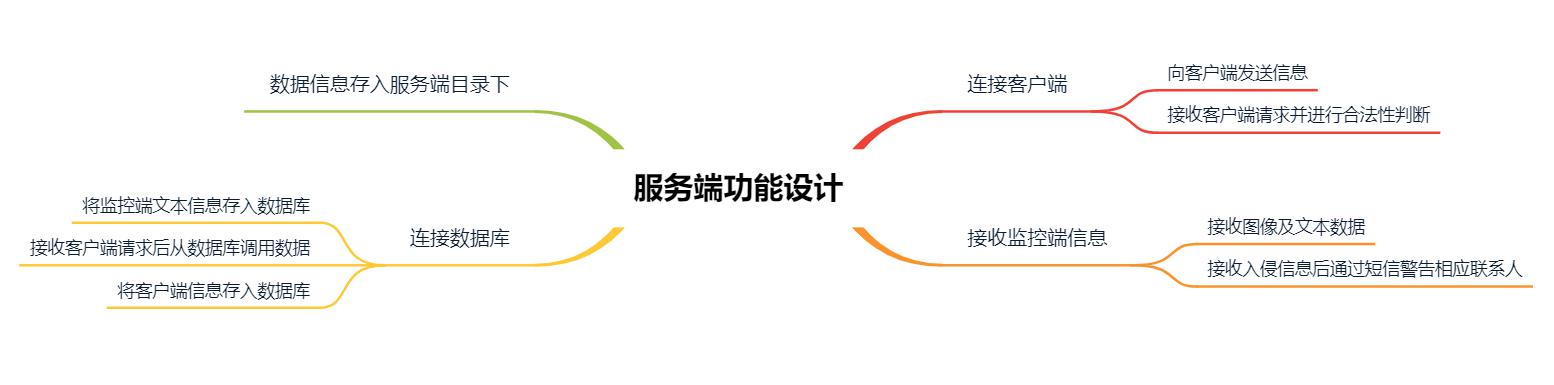
\includegraphics{img/3.jpg}
	\caption{服务器功能示意图}\label{fig:fig3}
\end{figure}
如\textbf{图\ref{fig:fig3}}所示,服务器的主要功能需求为
\newpage
\begin{enumerate}
	\item 持续监听来自监控端的连接请求,接收来自监控端的数据(支持断点续传);
	\item 将图片、文本信息信息存储至数据库;
	\item 通过短信、推送等方式告警客户联系人;
	\item 依据客户端指令调取数据库信息并反馈。
	
\end{enumerate}
\subsection{客户端}
\begin{figure}[!htbp]
	\centering
	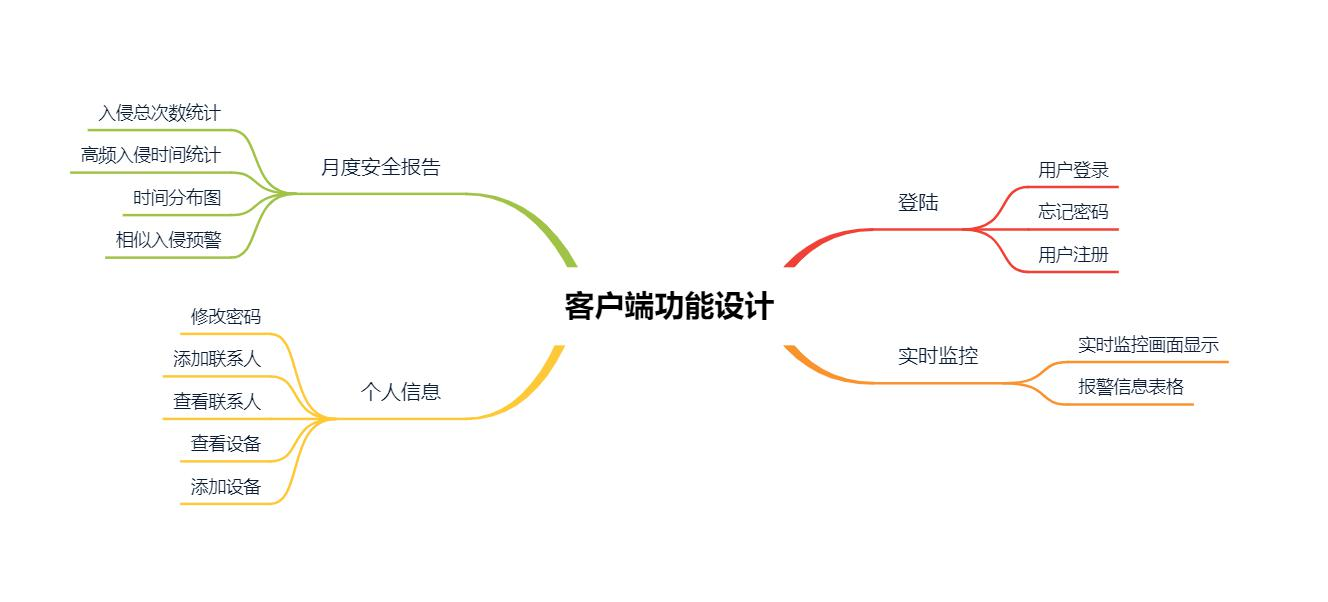
\includegraphics{img/4.jpg}
	\caption{客户端功能示意图}\label{fig:fig4}
\end{figure}
如\textbf{图\ref{fig:fig4}}所示,客户端的主要功能需求为
\newpage
\begin{enumerate}
	\item 用户注册/登录,核实监控端设备序列号;
	\item 修改个人信息,包括但不限于修改密码、添加联系人等;
	\item 查看实时监控画面、报警信息和月度安全报告;
	\item 设置安全时段。
	
\end{enumerate}

\section{系统架构设计}
\subsection{客户端-服务器 $\;$——$\;$三层B/S架构}
在客户端和服务器架构中,客户端对服务器发出请求并处理系统环境中的输入,而服务器是需要响应客户请求的应用程序。这种架构具有只需要便宜的硬件,可以有效使用网络系统,易于添加新服务器或升级现有的服务器等优点。

正如上一节所分析的,用户需要通过 OWL 入侵检测系统了解到监控范围内(如仓库、博物馆)的实时图像和发生入侵时的相关数据(包括捕获的图像,入侵物的信息等),并可通过系统启动或关闭监控设备。这一用户需求,可以抽象为用户向系统发出请求,系统根据用户的请求作出不同的响应,客户端和服务器架构可以很好地满足这一功能性需求,即用户可以通过系统提供的客户端向服务器发出指令,服务器作系统中数据的传输枢纽和处理、存储中心,可以对客户端发出的指令作出相应。综上所述,客户端和服务器架构适用于本系统。

但以应用程序作为客户端的架构,有着网络负载高、配置管理复杂和安全性复杂的缺点。例如,对于每一台需要安装客户端应用的终端(如 PC机,移动设备等),都需要按照用户手册安装必要的依赖环境和应用程序,而当客户端组件需要升级或进行维护时,每一台机器都需要安装更新包。当客户端抛出异常时,也需要系统的技术人员进行维护,大大增加了系统的维护成本。

而以浏览器作为客户端的系统架构,即 B/S 架构,由于浏览器几乎是每台用户终端的必备程序,因而具有配置管理简单(零安装),在服务器进行安全管理而不需要在浏览器进行维护,错误恢复容易,稳健性好等优势。因此,为了提高系统的易用性、安全性和可扩展性, B/S 架构为最优的解决方案。

三层客户端-服务器架构(B/S 架构)包括展示层、业务层和数据层,其中业务层分为业务逻辑层和数据访问层,其具体功能如下:
\begin{itemize}
\item 展示层:负责显示用户界面;
\item  业务层:负责访问数据层来获取、修改、删除数据并将结果发送到展示层;
\begin{itemize}
\item  业务逻辑层:在数据访问层之上,即业务逻辑层用到数据访问层的类和对象;
\item  数据访问层:负责处理数据并将数据传到业务逻辑层;
\end{itemize}
\item  数据层:数据库或数据源。
\end{itemize}

本项目的 B/S 架构设计图如图所示:

\begin{figure}[!htbp]
	\centering
	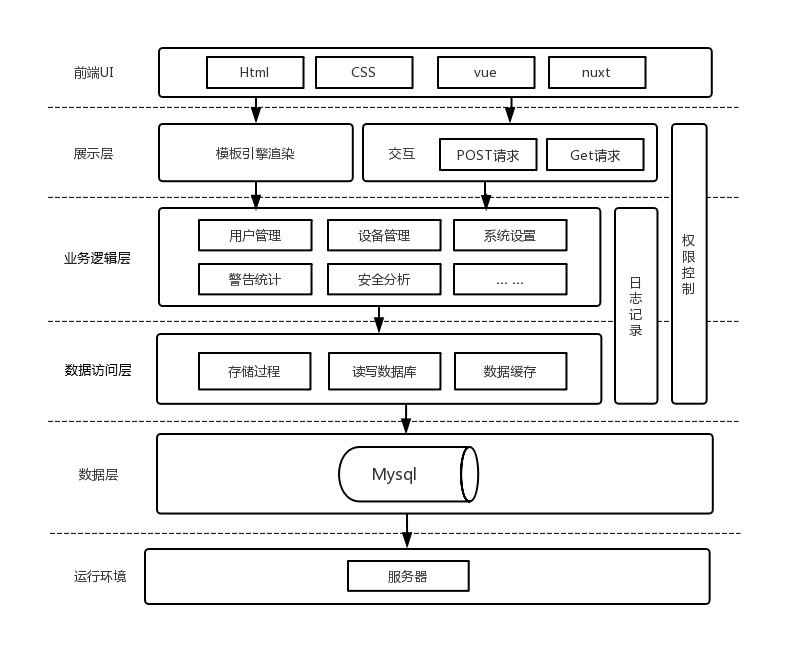
\includegraphics[scale=.8]{img/t1.jpg}
		\caption{OWL 入侵检测系统三层 B/S 架构设计图}
\end{figure}

\subsection{监控端-服务器$\;$——$\;$事件驱动架构}

事件驱动架构模式是一种非常流行的分布式异步架构模式,经常被用与构建高可伸缩性的应用程序。当然它也适合小型应用,复杂应用和规模比较大的应用。这种架构模式由一系列高度解耦的、异步接收和处理事件的单一职责的组件所组成。

事件驱动架构由两个主要的拓扑组成,分别是调停者拓扑(中断驱动模型)和代理者拓扑(广播模型)。调停者拓扑通过一个中央的调停者来编排各种处理步骤。然而代理者拓扑适用于那些当你想将事件链式的聚在一起但不使用中央调停者的情况。由于这两种模式特性以及实现均不一样,所以理解哪一个模式最适合你的实际情况是非常重要的。

事件驱动架构的核心是:
\begin{enumerate}
\item 事件发生则表示发生了一些事情(事件发生在这些事情后);
\item 事件被广播到它的监听代码中(多个监听程序可以共同处理一个事件)。
\end{enumerate}
在本入侵系统检测的项目中,“事件发生”对应着“入侵检测”的事件,“广播到监听代码”对应着“将检测结果发送给各个所有监听的子系统”。项目的拓扑结构如下图所示:

\begin{figure}[!htbp]
	\centering
	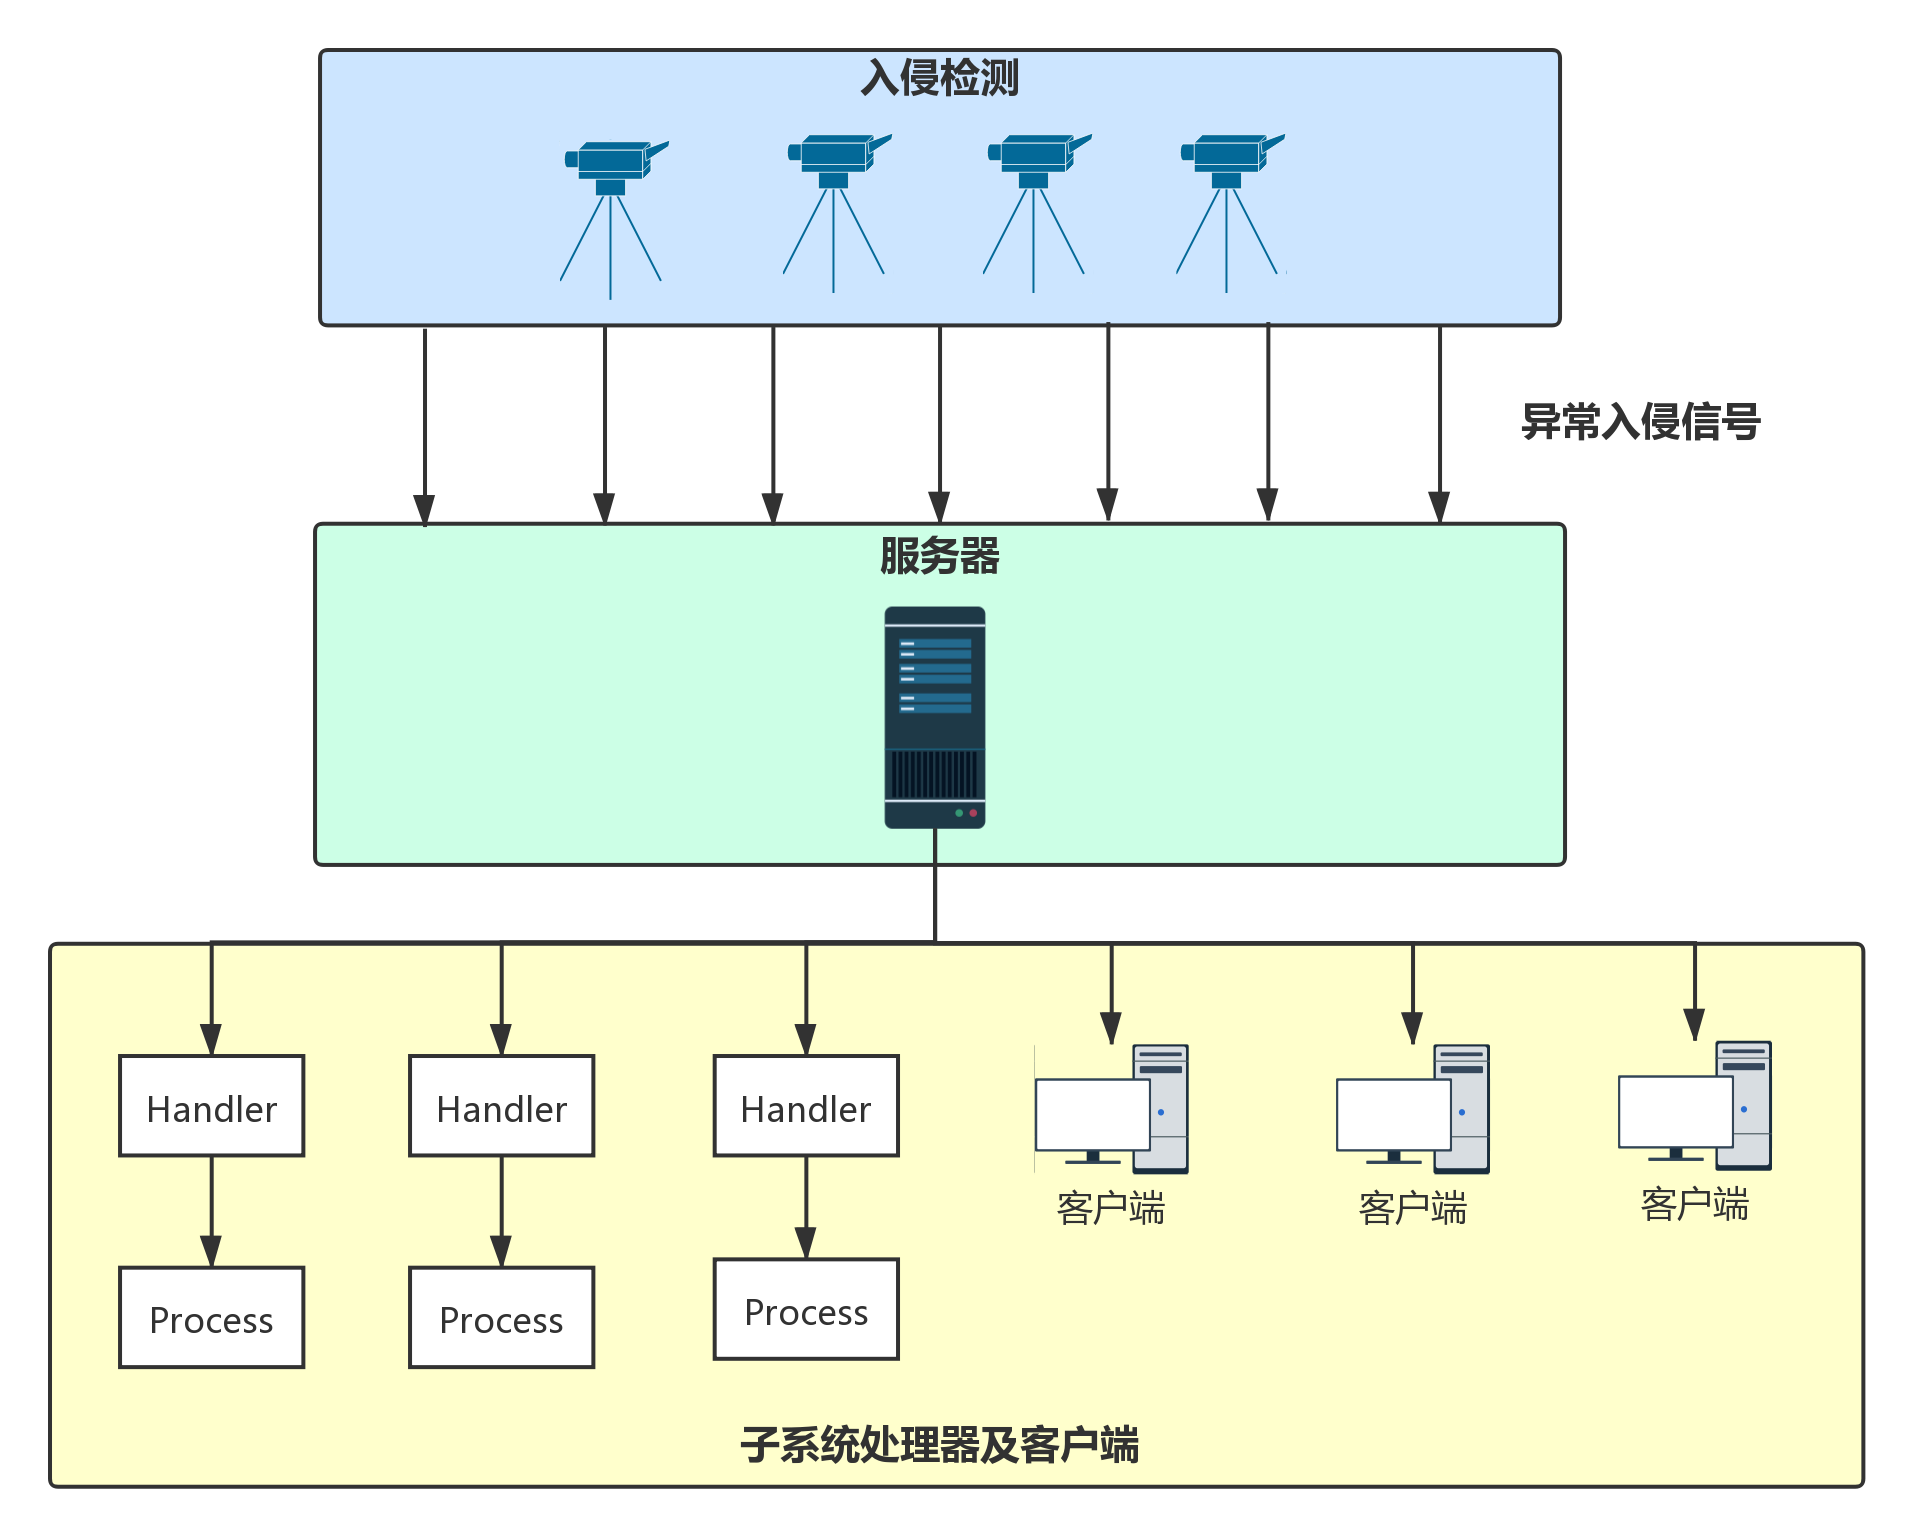
\includegraphics[scale=.25]{img/t2.png}
		\caption{OWL 入侵检测系统拓扑图}
\end{figure}

\begin{enumerate}
\item[(1)] \textbf{事件发生} 监测端的基本功能包括对入侵物体的检测、标注和分类存储等。Motion Detection 的实现方法有很多,本系统设计采用方法是Background subtraction,其基本原理实取一张静态的背景图(不包含要检测的移动物体),然后比较监控图像(包含移动物体)和背景图,找到不同区域,这个区域就是要检测的物体。

\item[(2)] \textbf{广播到监听代码} 本项目事件驱动架构部分的拓扑结构为调停者拓扑,即有物体入侵时,监控端先将事件发送给服务器端,由服务端作为中央调停者进行信息处理,并发送给各个子系统处理器及客户端。
\end{enumerate}

\subsubsection{事件发生——监控端发送入侵信号}
\begin{figure}[!htbp]
	\centering
	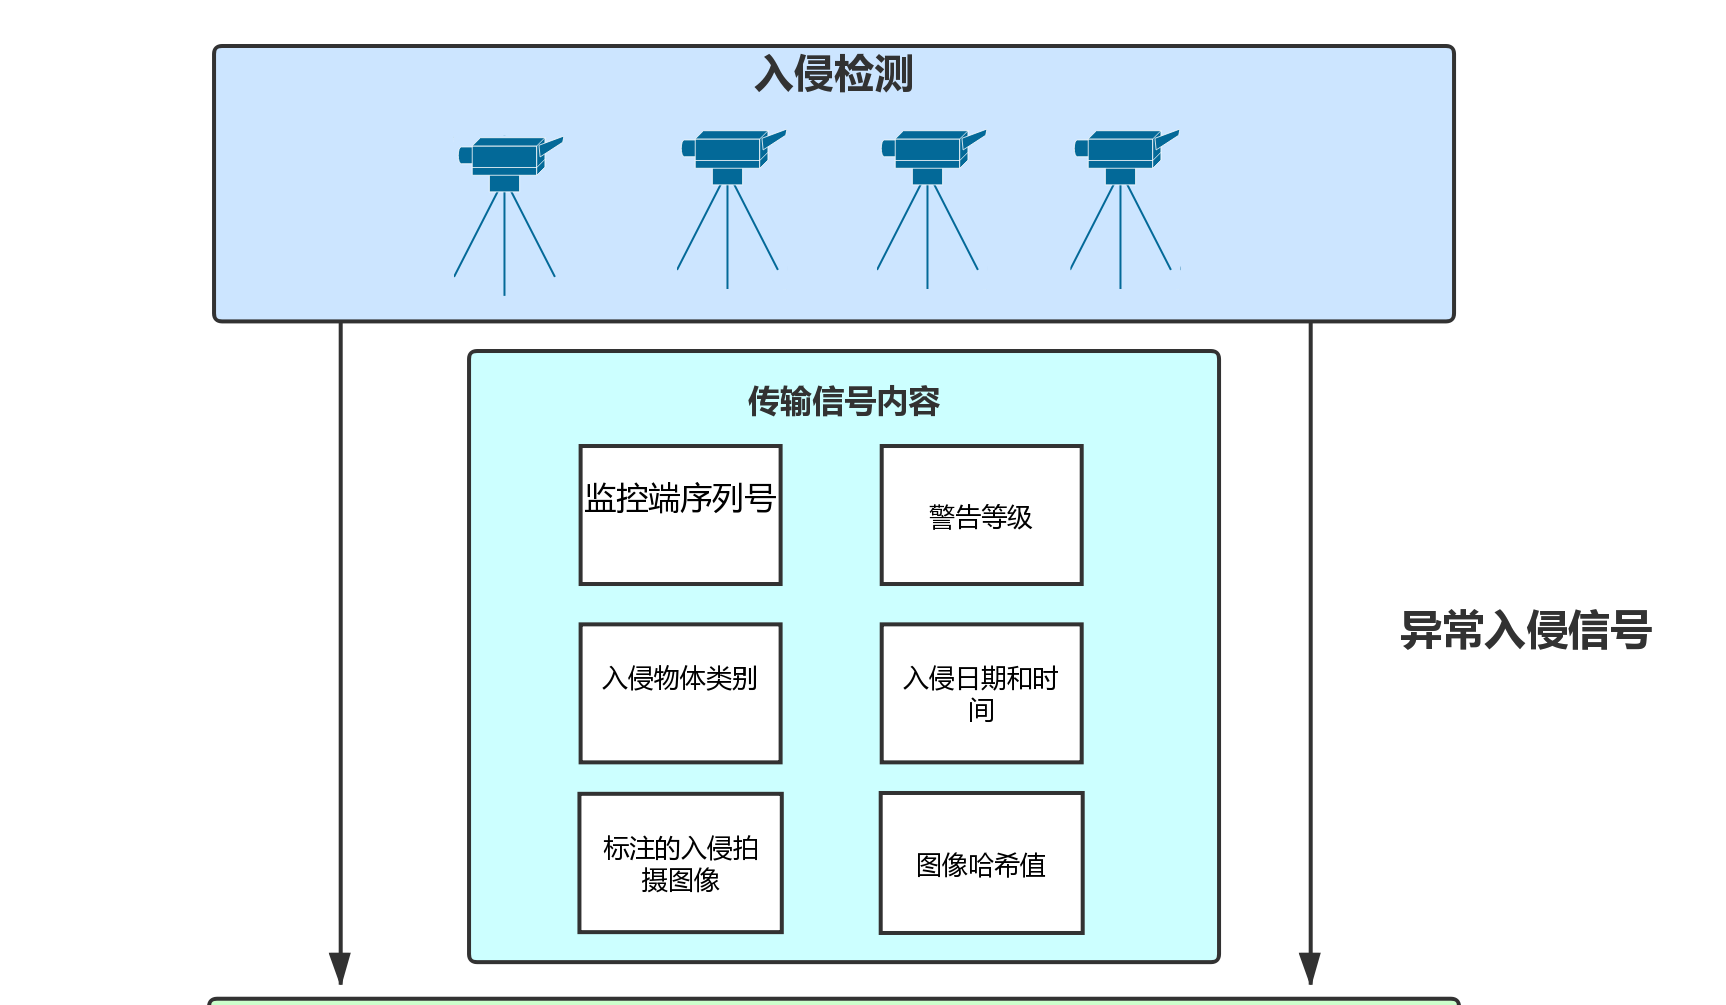
\includegraphics[scale=.25]{img/t3.png}
		\caption{监控端发送入侵信号事件模拟图}
\end{figure}

当检测到仓库内有移动物体时,监控端将监控端序列号、入侵日期和时间、标注的入侵拍摄图像、图像哈希值、入侵物体类别、警告等级等入侵警告数据和监控端基本数据发送到服务器端。其中图像以base64 和utf8 编码并使用hash处理以保证数据的安全性和完整性。所有数据以字典的数据类型写入json,发给服务器端。

\newpage 
\subsubsection{中央调停者——服务器端接受监控端数据}
\begin{figure}[!htbp]
	\centering
	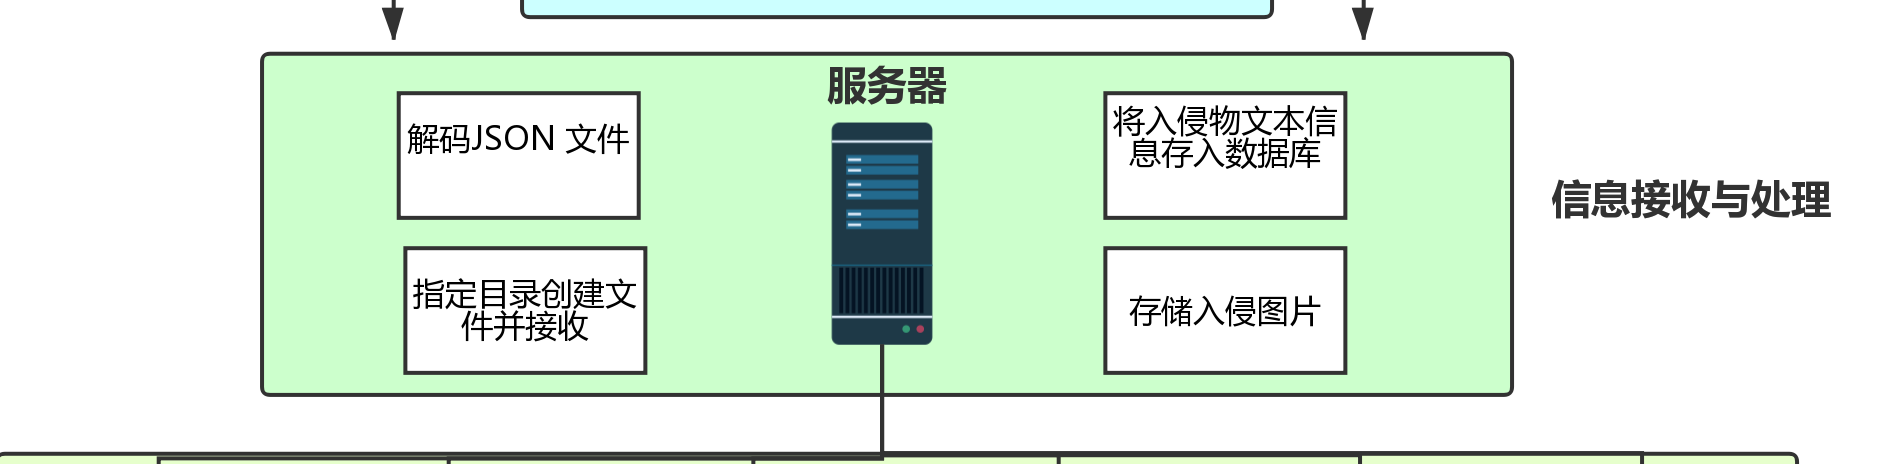
\includegraphics[scale=.25]{img/t4.png}
	\caption{服务器端接收监控端数据事件模拟图}
\end{figure}

服务端开启后持续监听来自监控端的连接请求,每收到一次请求后开启一个网络连接线程,与监控端完成一次数据交互,交互信息为由监控端对侵入物截取的图片及图片相关文本信息组成的信息包裹,一个包裹传输结束后即关闭该网络线程。服务器端将信息包裹存储到本地后,对信息包裹进行解析,提取文本信息并同步至本地数据库中,提取图片内容并存放至本地指定目录中。

\subsubsection{中央调停者——服务器端处理监控端数据}

服务器接受监控端的入侵信号后,会进行数据标注、识别和分类存储等处理,主要借由OpenCV 的图形处理功能。

\begin{enumerate}
	\item[(1)] \textbf{图片信息存储至本地}
	
	服务器端根据JSON 文件解码后得到的入侵时间、入侵物分类创建对应的文件目录,使用文件输出流对图片信息进行存储。
	
	\item[(2)] \textbf{文本信息存储至数据库}
	
	监控端传给服务端,且需要保存至数据库的信息为入侵物的信息,包括入侵时间、入侵物分类、入侵物危险等级、检测到入侵物的监控端标识符。首先在本地数据库中创建用来存放此类信息的表格,在后端通过数据库名称、数据库表单名称、数据库端口号、用户名、密码访问数据库,使用MYSOL 命令与句将解码JSON 文件的到的信息存储至数据库中。
\end{enumerate}

\newpage
\subsubsection{广播至处理器及客户端}
\begin{figure}[!htbp]
	\centering
	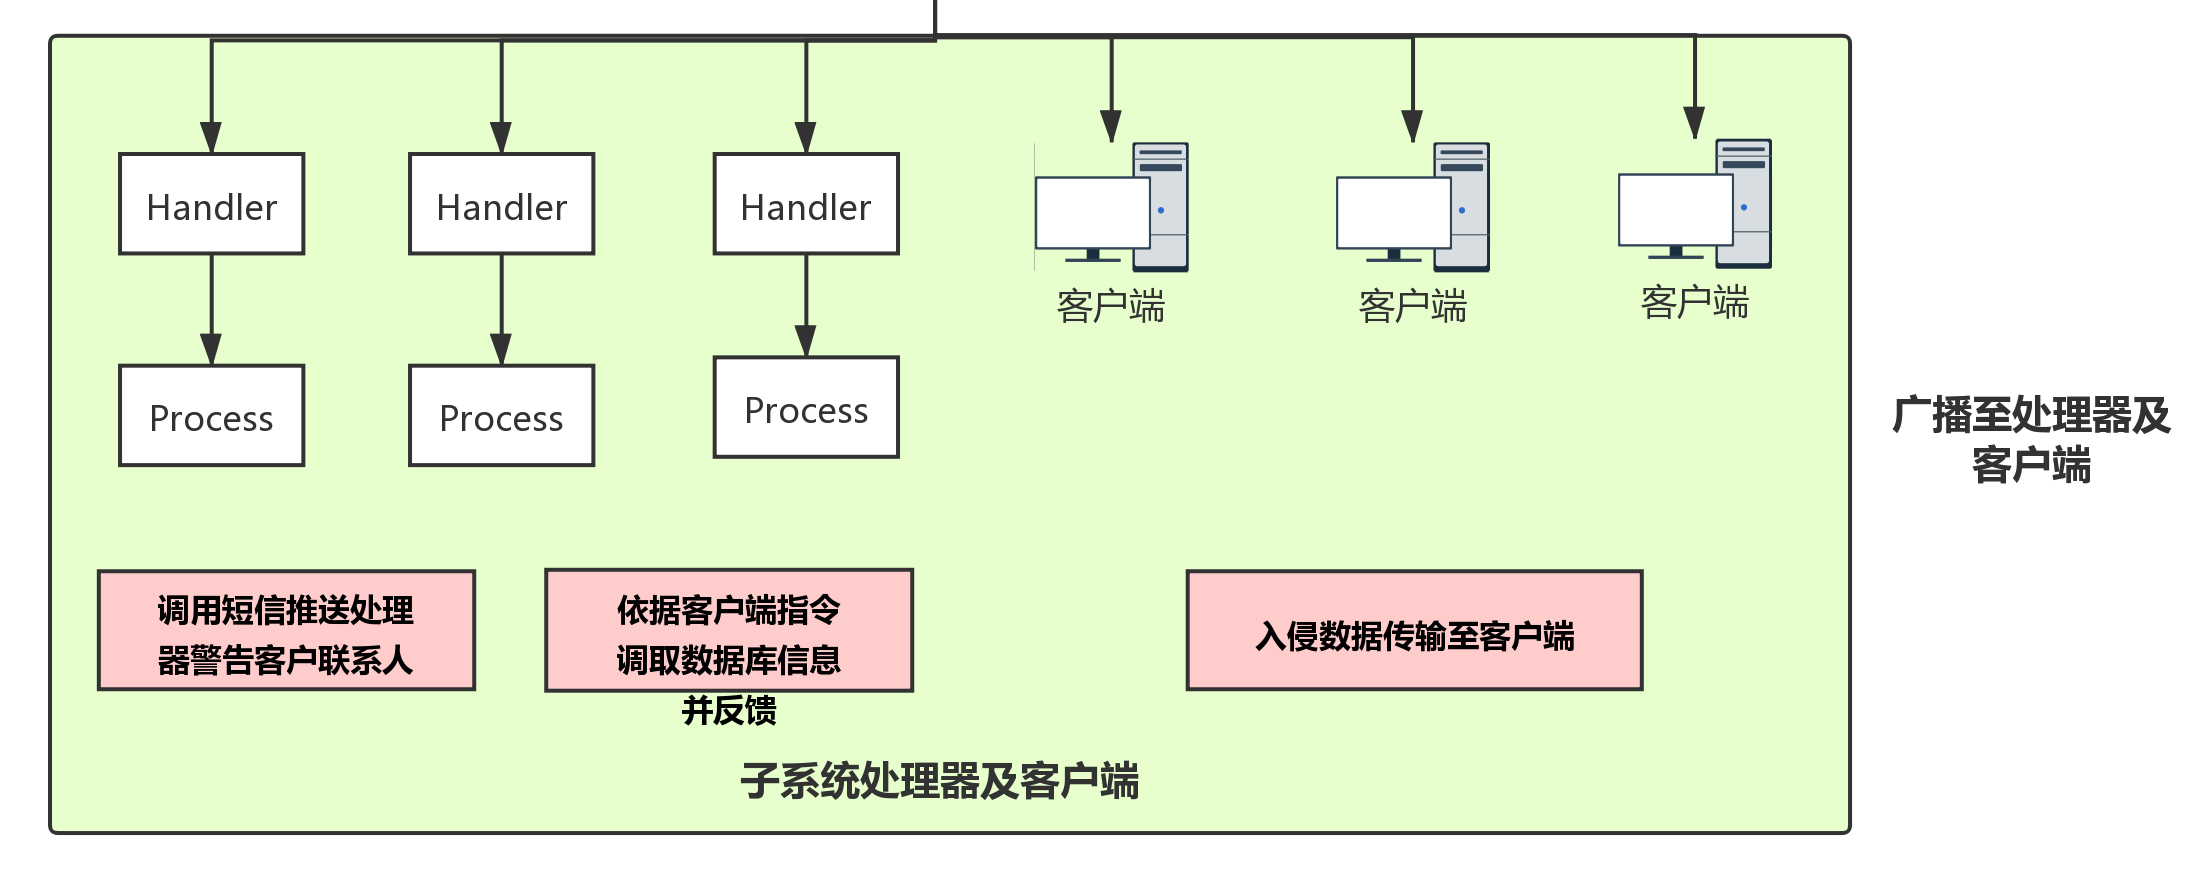
\includegraphics[scale=.2]{img/t5.png}
	\caption{广播至处理器及客户端图}
\end{figure}

\begin{enumerate}
	\item[(1)] \textbf{广播至客户端——入侵数据传输:}
	
	服务器端开启,等待前端客户访问前端网页,前端网页与服务器端通过Web Socket 连接并传送数据。使用Web Socket 的原因是方便实现服务端主动发送信息至网页,而非前端请求。服务器端根据客户端身份标识符在数据库中添加相关信息,或是提取相关信息反馈给客户端。当接收到监控端的入侵信息传输时,主动给监控端对应的客户端发送入侵物的相关信息。
	
	\item[(2)] \textbf{广播至处理器——调用短信推送处理器警告客户联系人}
	
	服务端接收到来自监控端的入侵信息后,判断当前时间是否属于安全时段,若是则不做处理,若不是则需要主动尝试将入侵信息传给客户端浏览器,且发送短信通知用户。后端发送短信的方式是依托于腾讯云服务,调用SmsSingleSender 接口,凭借AppID 及AppKey,使用通过审核的身份签名及短信正文模板发送给监控端对应的客户端联系人的手机号码。
	
	\item[(3)] \textbf{广播至客户端及调用处理器——依据客户端指令调取数据库信息并反馈}
	
	服务端Tomcat 服务器开启WebSocket,接收客户端浏览器连接后发来的身份标识符及指令,在后端以身份标识符为键值,以对应客户端WebSocket 对象为值将二者添加至Map 中,以便后续主动发送对应信息给对应客户。服务端根据指令代码,将指令中用户输入内容与数据库中存储内容进行比对,或是提取数据库中向相关信息,再将比对结果或是数据库信息反传给客户端。
\end{enumerate}

\subsubsection{总结}
综上所述,在入侵检测-服务器接收数据与处理-广播至客户端及处理器的过程中,项目使用了事件驱动架构的调停者拓扑(中断驱动模型)结构。
\begin{figure}[!htbp]
	\centering
	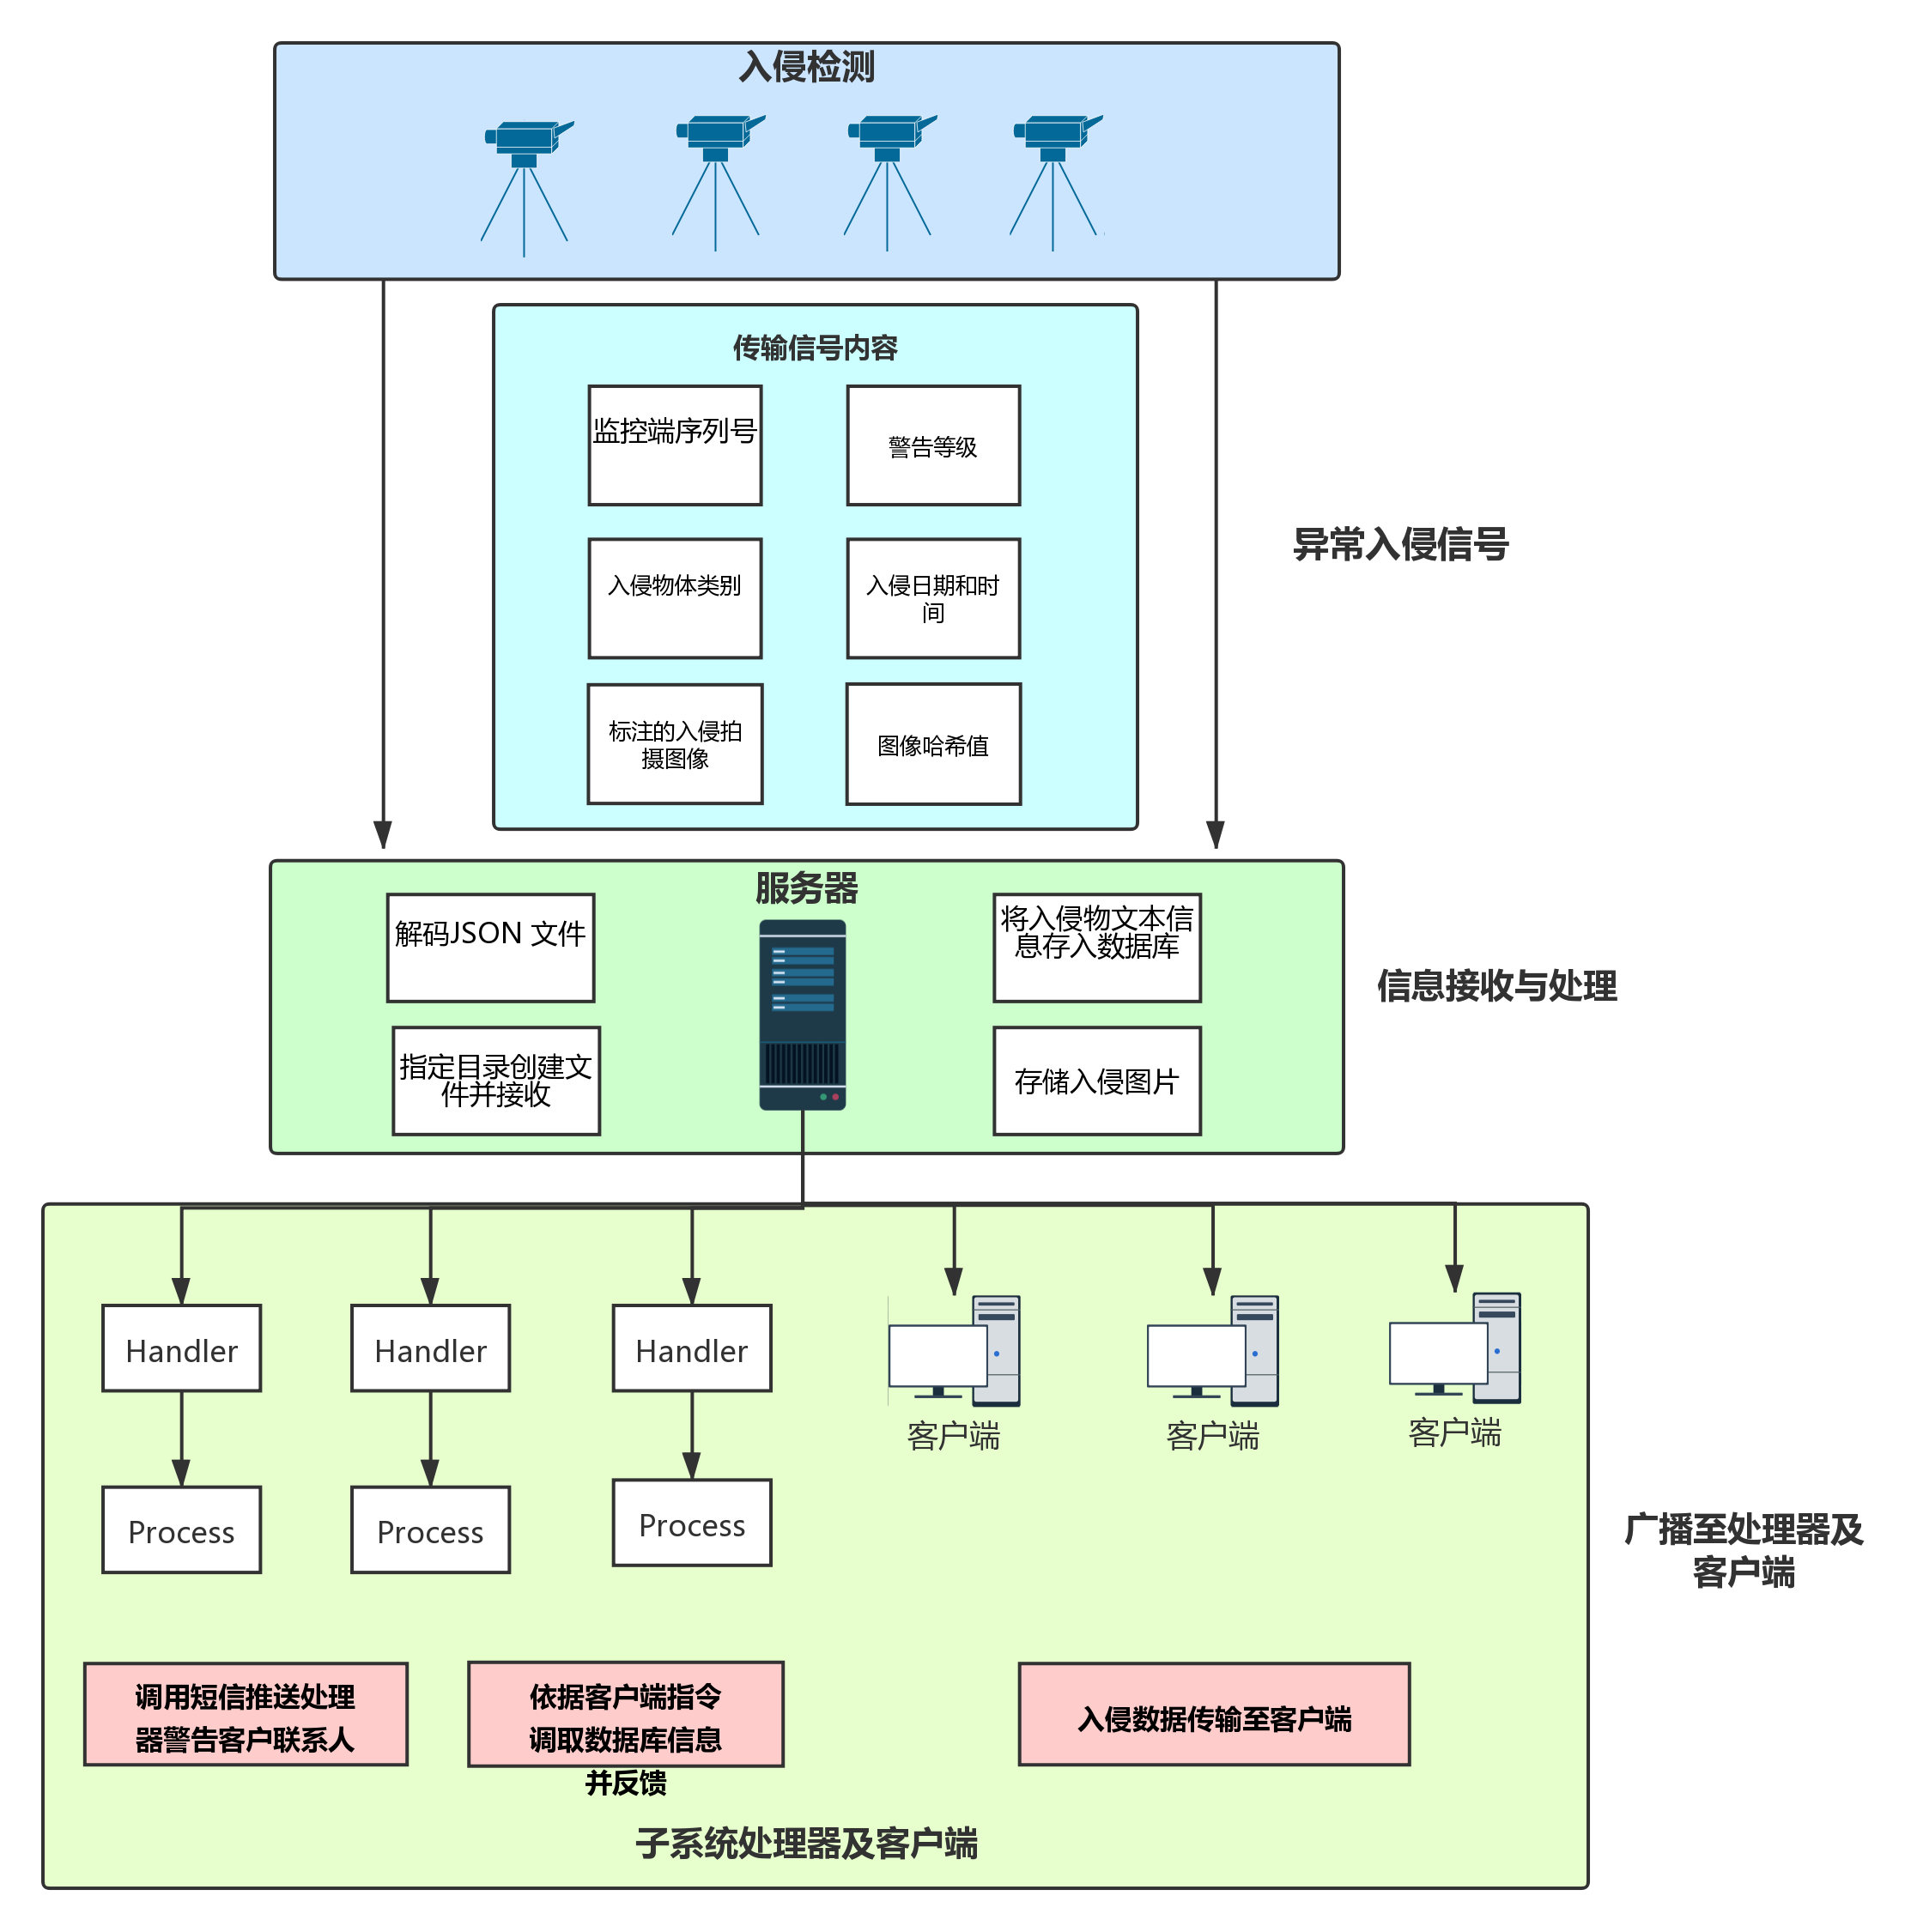
\includegraphics[scale=.2]{img/t6.png}
	\caption{OWL 入侵监测系统事件驱动架构设计图}
\end{figure}

\subsection{MVVM 设计模式}
MVVM(Model-View-ViewModel) 是一种软件架构设计模式,是一种简化用户界面的事件驱动编程方式,由 John Gossman 于2005年发表。

按照 MVVM 的设计思想,总体上分为三大块,分别是 View 层、ViewModel 层、Model 层。
\begin{itemize}
\item View 层负责视图逻辑;
\item Model 层负责处理数据逻辑;
\item ViewModel 层负责处理业务逻辑,为 View 层提供数据源;
\end{itemize}
其整体结构大体如下:
\begin{figure}[!htbp]
	\centering
	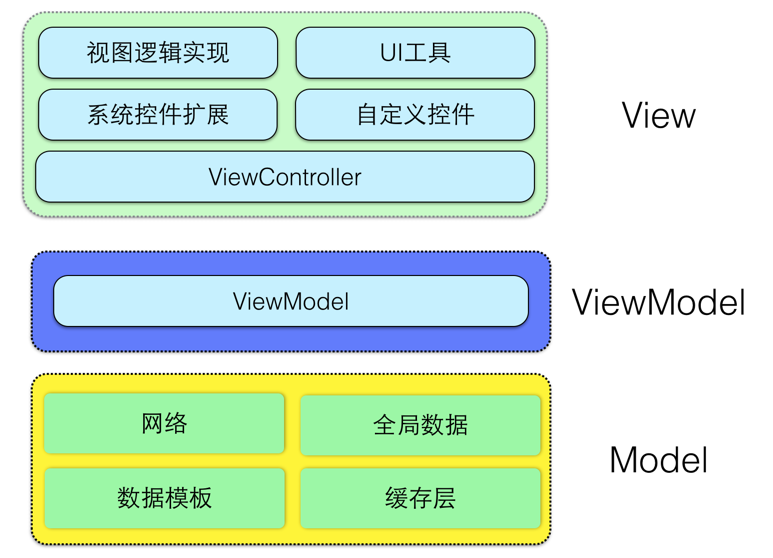
\includegraphics[scale=.75]{img/t7.png}
	\caption{OWL 入侵监测系统事件驱动架构设计图}
\end{figure}

MVVM 的核心是数据驱动即 ViewModel,ViewModel 是 View 和 Model 的关系映射。ViewModel 类似中转站(Value Converter),负责转换 Model 中的数据对象,使得数据变得更加易于管理和使用。MVVM 本质就是基于操作数据来操作视图进而操作 DOM,借助于 MVVM 无需直接操作 DOM,开发者只需完成包含声明绑定的视图模板,编写 ViewModel 中有业务,使得 View 完全实现自动化。
\newpage
出于对“入侵监控”这一需求的考虑,直面用户的 View 部分需要随数据及时更新,每次入侵出现都会需要及时的更新进 View,而当用户的操作导致 View 发生变化,开发者同样需要将变化的数据同步到 Model 中,采用 MVVM 的架构模式可以轻松简化这一繁琐的过程。在 MVVM 架构下,View 和 Model 之间并没有直接的联系,而是通过 ViewModel 进行交互,Model 和 ViewModel之间的交互是双向的。因此 View 数据的变化会同步到 Model 中,而 Model数据的变化也会立即反应到 View 上,简化了 API 和 DOM 操作。

本项目客户端的每一部分组件均被拆解成 View-Model-ViewModel 结构,$<$template$>$ $<$/template$>$ 标签中集中存放界面部分代码,处理视图逻辑;$<$script$><$/script$>$ 标签中处理业务逻辑,为 View 部分提供数据源,而 data(){} 中则存放和数据库中数据相对应的数据,负责处理数据逻辑。以 messageTable 组件为例,组件部分代码如下:

\begin{figure}[!htbp]
	\centering
	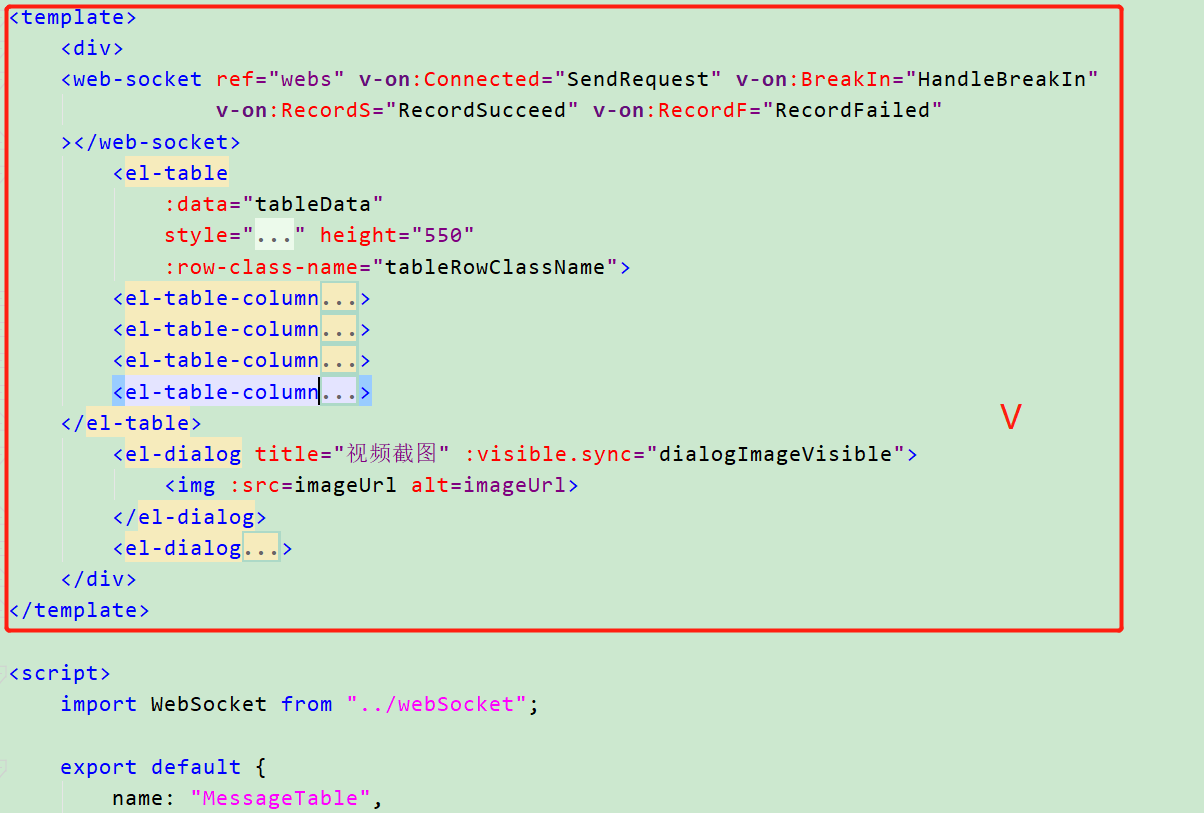
\includegraphics[scale=.5]{img/t8.png}
	\caption{示例代码图(一)}
\end{figure}

\begin{figure}[!htbp]
	\centering
	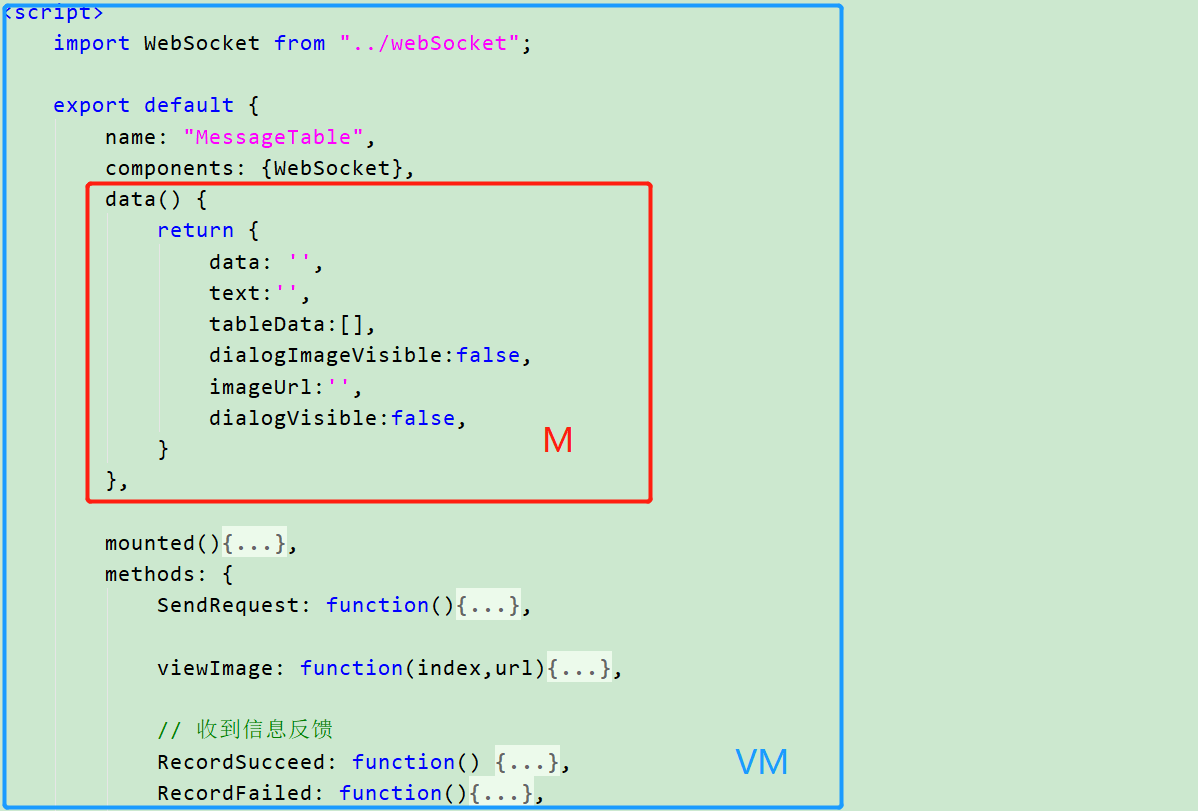
\includegraphics[scale=.6]{img/t9.png}
	\caption{示例代码图(二)}
\end{figure}
\newpage
如图中标注,data 部分的数据与 template 绑定,数据变化可以渲染到视图;而整个script部分则对业务逻辑进行处理,通过声明式的数据绑定来实现 View 的分离,完全解耦 View,实现 UI 和功能的解耦合。

\subsection{仓库模式}
本系统采用 MySQL 数据库作为中央仓库,轻量、快速,且功能强大,移植性较好;本系统中央数据库由用户的基本信息表、报警信息表构成。基本信息表存储设备的序列号、序列密码,当购买了设备的用户根据设备上序列号和序列密码就可以注册自己的账号和密码,服务器将此账号和密码也存入基本信息表中。还可以添加联系人的姓名和电话号码存入基本信息表中。报警信息表存储用户ID、报警的日期、具体时间、危险等级、危险详情。中央仓库存储所有的数据,前段和监控端都通过服务器与中央仓库交互,这样就能实现共享数据。
\newpage
\subsubsection{数据库表设计}

\begin{table}[!htbp]
	\centering
	\caption{数据库表设计}
	\label{tab:my-table}
	\begin{tabular}{|l|l|l|l|}
		\hline
		序号 & 表名    & Code         & 描述                 \\ \hline
		1  & 用户表   & basicInfo    & 存储用户属性的数据库表        \\ \hline
		2  & 报警信息表 & alarmMessage & 存储所有报警信息和报警图片的数据库表 \\ \hline
	\end{tabular}
\end{table}

\subsubsection{数据库各表字段}

\begin{table}[!htbp]
	\centering
	\caption{数据库各表字段}
	\label{tab:my-table}
	\begin{tabular}{|p{3cm}|p{3cm}|p{8cm}|}
		\hline
		\multicolumn{3}{|c|}{\begin{tabular}[c]{@{}c@{}}用户表\\ basicInfo\end{tabular}} \\ \hline
		字段名                        & 数据类型                & 说明                         \\ \hline
		serialID                   & Varchar             & 设备序列号                      \\ \hline
		serialPassword             & Varchar             & 设备密码                       \\ \hline
		userID                     & Varchar             & 用户名,唯一标识用户身份的主键            \\ \hline
		userPassword               & Varchar             & 用户密码                       \\ \hline
		userName1                  & Varchar             & 联系人1                       \\ \hline
		userTel1                   & Varchar             & 联系电话1                      \\ \hline
		userName2                  & Varchar             & 联系人2                       \\ \hline
		userTel2                   & Varchar             & 联系电话2                      \\ \hline
		userName3                  & Varchar             & 联系人3                       \\ \hline
		userTel3                   & Varchar             & 联系电话3                      \\ \hline
		userName4                  & Varchar             & 联系人4                       \\ \hline
		userTel4                   & Varchar             & 联系电话4                      \\ \hline
		userName5                  & Varchar             & 联系人5                       \\ \hline
		userTel5                   & Varchar             & 联系电话5                      \\ \hline
		status                     & Varchar             & 状态                         \\ \hline
	\end{tabular}
\end{table}

\begin{table}[!htbp]
	\centering
	\caption{数据库各表字段}
	\label{tab:my-table}
		\begin{tabular}{|p{3cm}|p{3cm}|p{8cm}|}
		\hline
		\multicolumn{3}{|c|}{\begin{tabular}[c]{@{}c@{}}报警信息表\\ alarmMessage\end{tabular}} \\ \hline
		字段名                        & 数据类型                   & 说明                           \\ \hline
		id                         & Varchar                & 用户id                         \\ \hline
		date                       & Varchar                & 报警日期包括年,月                    \\ \hline
		time                       & Varchar                & 报警具体时间(日,时,分,秒)              \\ \hline
		riskLevel                  & Varchar                & 危险级别                         \\ \hline
		details                    & Varchar                & 详情                           \\ \hline
		create\_time               & timestamp              & 插入记录的当前时间                    \\ \hline
		URL                        & Varchar                & 报警图片的本地url地址                 \\ \hline
		PATH                       & Varchar                & 报警图片的url链接                   \\ \hline
	\end{tabular}
\end{table}
\newpage
\subsubsection{概念模型设计}
\begin{figure}[!htbp]
	\centering
	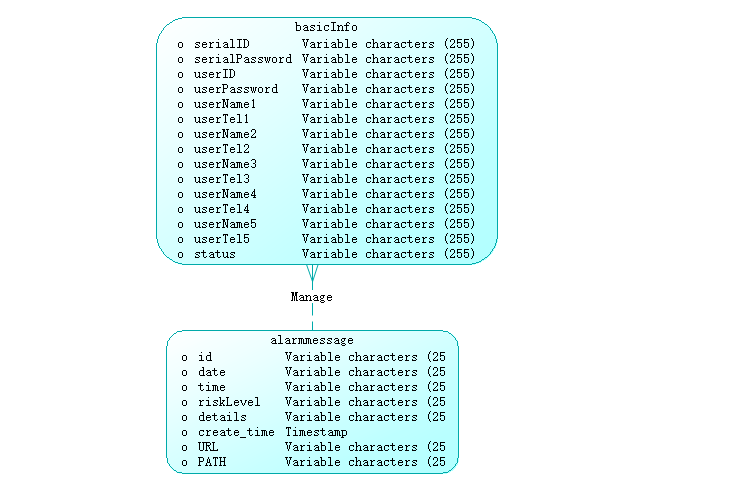
\includegraphics[scale=.9]{img/t10.png}
	\caption{概念模型设计图}
\end{figure}

\subsubsection{逻辑模型设计}
\begin{figure}[!htbp]
	\centering
	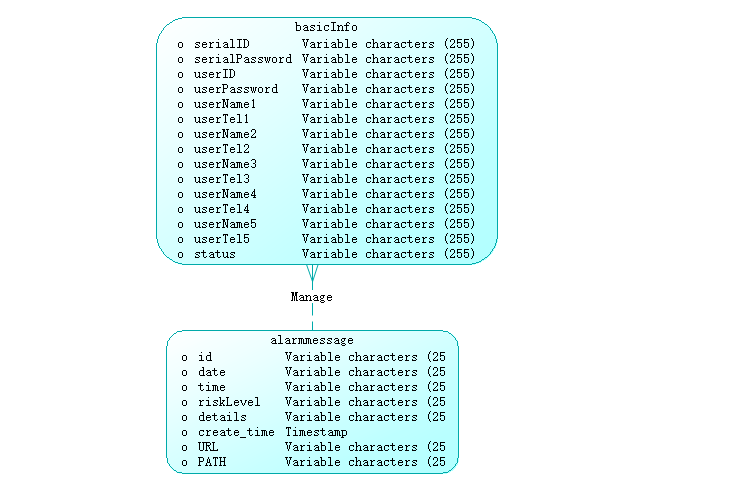
\includegraphics[scale=.9]{img/t11.png}
	\caption{逻辑模型设计图}
\end{figure}

\subsubsection{物理模型设计}
\begin{figure}[!htbp]
	\centering
	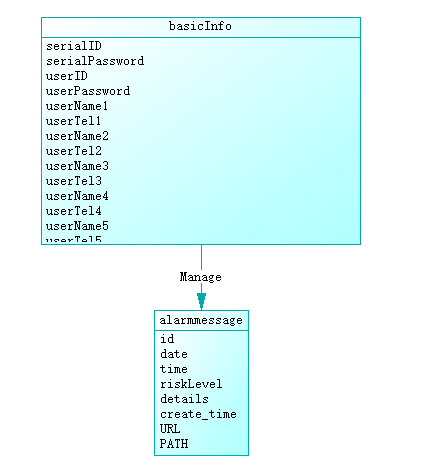
\includegraphics[scale=.9]{img/t12.png}
	\caption{物理模型设计图}
\end{figure}

\subsubsection{系统仓库模式架构}
\begin{figure}[!htbp]
	\centering
	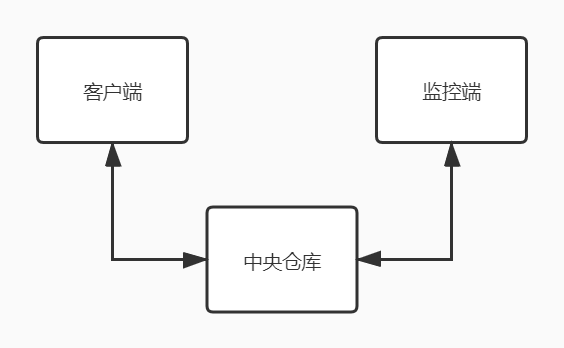
\includegraphics[scale=.8]{img/t13.png}
	\caption{OWL 入侵监测系统仓库模式架构图}
\end{figure}
\newpage
\section{系统架构设计图}
综上所述,OWL 入侵监测系统的系统架构模式如下图所示。

\begin{figure}[!htbp]
	\centering
	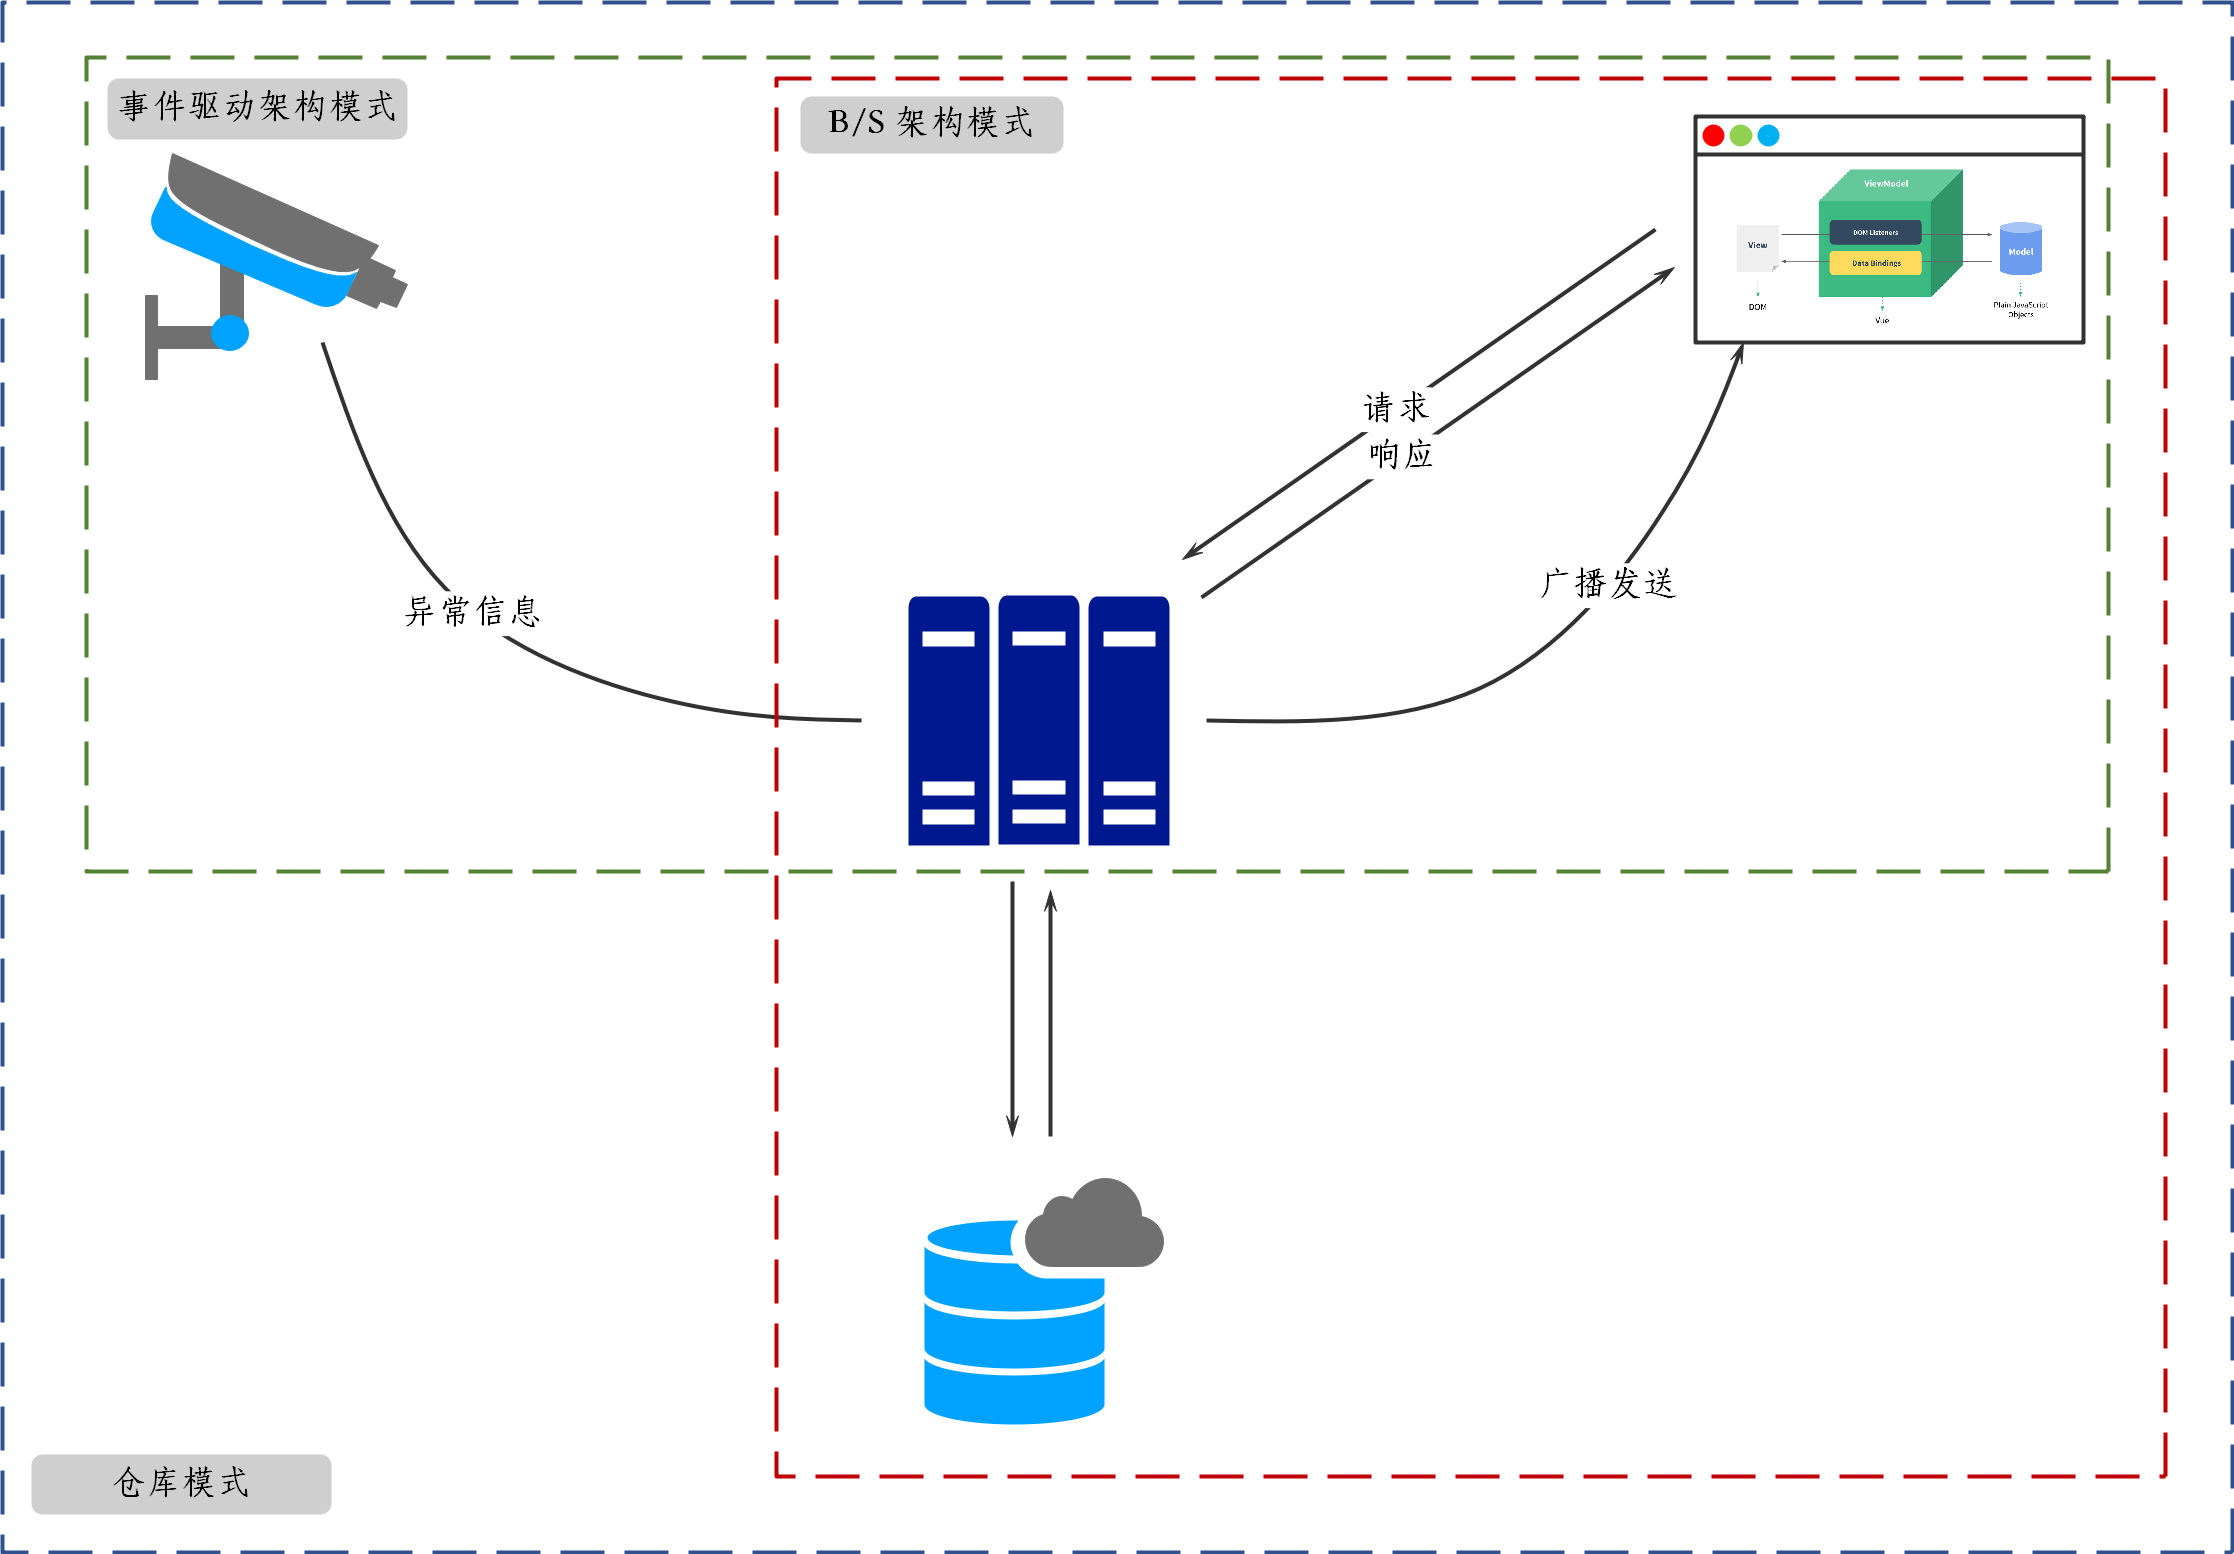
\includegraphics[scale=.28]{img/t14.png}
	\caption{OWL 入侵监测系统架构图}
\end{figure}
\end{document}